%%%%%%%%%%%%%%%%%%%%%%%%%%%%%%%%%%%%%%%%%%%%%%%%%%%%%%%%%%%%%%%%%%%%%%%% 
%%%%%%%%%%%%%%%%%%%%%%%%%%%%%%%%%%%%%%%%%%%%%%%%%%%%%%%%%%%%%%%%%%%%%%%% 
\begin{frame}[fragile=singleslide]
  \frametitle{Hands-On 6 : Random number generator with Kokkos}

  \begin{itemize}
  \item Activity: \textcolor{red}{\bf Estimating Pi via Monte Carlo}
  \item purpose: learn to use the {\bf random number generator} features (built-in Kokkos)
  \item Draw random points in $[0,1]^2$ and compute the fraction of points inside the unit circle:
    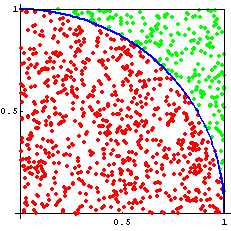
\includegraphics[width=2.5cm]{images/MonteCarloPiMod_gr_25}
  \item These generators are based on Vigna, Sebastiano (2014). {\it An experimental exploration of Marsaglia's xorshift generators, scrambled.} \myurl{http://arxiv.org/abs/1402.6246}
  \item Use code in \texttt{code/handson/6/compute\_pi}; read \texttt{readme} file; fill the holes
  \item Which compute pattern will you use ? \texttt{parallel\_for}, \texttt{parallel\_reduce}, \texttt{parallel\_scan} ?
  \end{itemize}
  
\end{frame}